% 
% ---------------------------------------------------------------
% Copyright (C) 2012-2018 Gang Li
% ---------------------------------------------------------------
%
% This work is the default powerdot-tuliplab style test file in TULIP Lab and may be
% distributed and/or modified under the conditions of the LaTeX Project Public
% License, either version 1.3 of this license or (at your option) any later
% version. The latest version of this license is in
% http://www.latex-project.org/lppl.txt and version 1.3 or later is part of all
% distributions of LaTeX version 2003/12/01 or later.
%
% This work has the LPPL maintenance status "maintained".
%
% This Current Maintainer of this work is Gang Li.
%
%

% Document Class
\documentclass[
size=12pt,
paper=smartboard,  %a4paper, smartboard, screen
mode=present, 		%present, handout, print
display=slides, 	% slidesnotes, notes, slides
style=tuliplab,  	% TULIP Lab style
pauseslide,
fleqn,leqno]{powerdot}

\usepackage{amssymb}
\usepackage{amsmath} 
\usepackage{rotating}
\usepackage{graphicx}
\usepackage{boxedminipage}
\usepackage{media9}
\usepackage{rotate}
\usepackage{calc}
\usepackage[absolute]{textpos}
\usepackage{psfrag,overpic}
\usepackage{fouriernc}
\usepackage{pstricks,pst-node,pst-text,pst-3d,pst-grad}
\usepackage{moreverb,epsfig,color,subfigure}
\usepackage{color}
\usepackage{pstricks}
\usepackage{pstricks-add}
\usepackage{pst-text}
\usepackage{pst-node, pst-tree}
\usepackage{booktabs}
\usepackage{etex}
\usepackage{breqn}
\usepackage{multirow}
\usepackage{gitinfo2}
\usepackage{subfigure}
% \usepackage{pst-rel-points}

\usepackage{listings}
\lstset{frameround=fttt, 
	frame=trBL, 
	stringstyle=\ttfamily,
	backgroundcolor=\color{yellow!20},
	basicstyle=\footnotesize\ttfamily}
\lstnewenvironment{code}{
	\lstset{frame=single,escapeinside=`',
		backgroundcolor=\color{yellow!20},
		basicstyle=\footnotesize\ttfamily}
}{}


\usepackage{hyperref}
\hypersetup{ % TODO: PDF meta Data
	pdftitle={Flip00 Presentation},
	pdfauthor={Baobao Song},
	pdfpagemode={FullScreen},
	pdfborder={0 0 0}
}


% \usepackage{auto-pst-pdf}
% package to show source code

\definecolor{LightGray}{rgb}{0.9,0.9,0.9}
\newlength{\pixel}\setlength\pixel{0.000714285714\slidewidth}
\setlength{\TPHorizModule}{\slidewidth}
\setlength{\TPVertModule}{\slideheight}
\newcommand\highlight[1]{\fbox{#1}}
\newcommand\icite[1]{{\footnotesize [#1]}}

\newcommand\twotonebox[2]{\fcolorbox{pdcolor2}{pdcolor2}
	{#1\vphantom{#2}}\fcolorbox{pdcolor2}{white}{#2\vphantom{#1}}}
\newcommand\twotoneboxo[2]{\fcolorbox{pdcolor2}{pdcolor2}
	{#1}\fcolorbox{pdcolor2}{white}{#2}}
\newcommand\vpspace[1]{\vphantom{\vspace{#1}}}
\newcommand\hpspace[1]{\hphantom{\hspace{#1}}}
\newcommand\COMMENT[1]{}

\newcommand\placepos[3]{\hbox to\z@{\kern#1
		\raisebox{-#2}[\z@][\z@]{#3}\hss}\ignorespaces} 


%%%%%%%%%%%%%%%%%%%%%%%%%%%%%%%%%%%%%%%%%%%%%%%%%%%%%%%%%%%%%%%%%%%%%%%%
% title
% TODO: Customize to your Own Title, Name, Address
%
\title{Flip00 Presentation}
\author{
	Baobao Song
	\\
	Hunan University 
	% \href{mailto:gangli@acm.org}{gangli@acm.org}
	% \and % more authors
}
\date{\today}


% Customize the setting of slides
\pdsetup{
	% TODO: Customize the left footer, and right footer
	rf=\href{http://www.tulip.org.au}{
		Last Changed: 2020-9-18
	},
	cf={Flip00 Presentation},
}


% Starts the document
\begin{document}
	
	\maketitle 
	
	%%==========================================================================================
	%%
	\begin{slide}[toc=,bm=]{Table of Content}
		\tableofcontents[type=1,content=futuresections]
		%  \tableofcontents[content=sections]
	\end{slide}
	%%
	%%==========================================================================================
	
	\section{Problem}
	
	\begin{slide}{Description and Evalution}
		\twotonebox{Description}{\parbox{.8\textwidth}
			{Predict Future Sales by giving a time-series dataset consisting of daily sales data}}
		\\
		\vbox{}
		\twotonebox{Evalution}{\parbox{.815\textwidth}
			{Root mean squared error (RMSE)
				\\True target values are clipped into [0,20] range}}
	\end{slide}
	
	
	\section{Data Processing}
	
	
	%%==========================================================================================
	%%
	\begin{slide}[toc=Basic Information of Data]{Basic Information of Data}
		\smallskip
		\centerline{\normalsize{Table 1:Data}}
		\begin{tabular}{cp{7cm}p{7cm}}
			\hline
			Name&Description&Attribute\\
			\hline
			sales\_train.csv& Training set(data from January 2013 to October 2015)&date,date_block_num,shop_id, item_id, item_price,item_cnt_day\\
			test.csv& Test set(Predict sale in November 2015) & ID,shop_id,item_id\\
			items.csv& Supplementary information of products &item_name,item_id,item_category_id\\
			shops.csv& Supplementary information of shops & shops_name,shops_id\\
			item_categories.csv& Supplementary information of item categories & item_categories_name,item_categories_id\\
			sample_submission.csv& Format of submission & ID,item_cnt_month\\
			\hline
		\end{tabular}
		\begin{itemize}
			\bigskip
			\item 
			There are 2935849 lines in train set\\
			There are 214200 lines in test set\\
			\vbox{}
			\item 
			There are 21807 unique items in train set\\
			There are 60 unique shops in train set\\
			There are 5100 unique items in test set\\
			There are 42 unique shops in test set
		\end{itemize}
	\end{slide}
	%%
	%%==========================================================================================
	
	%%==========================================================================================
	%%
	\begin{slide}[toc=Missing Value and NaN Value]{Missing Value and NaN Value}
		
		\begin{figure}[htb]
			\centering
			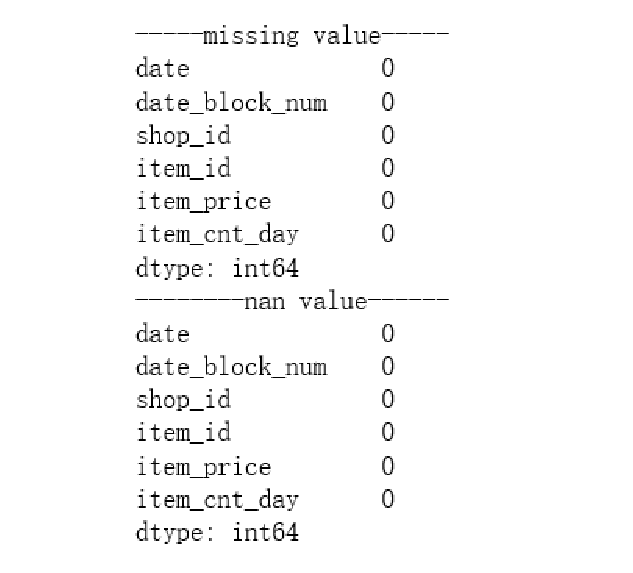
\includegraphics[width=12cm, height=10cm]{figures/miss.eps}\\
			\caption{Missing Value and NaN Value
			}\label{straddltimeScale}
		\end{figure}
	\end{slide}
	%%
	%%==========================================================================================
	%%==========================================================================================
	%%  
	\begin{slide}[toc=Outliers and Duplicate Data]{Outliers and Duplicate Data}
		\begin{figure}[htb]
			\centering
			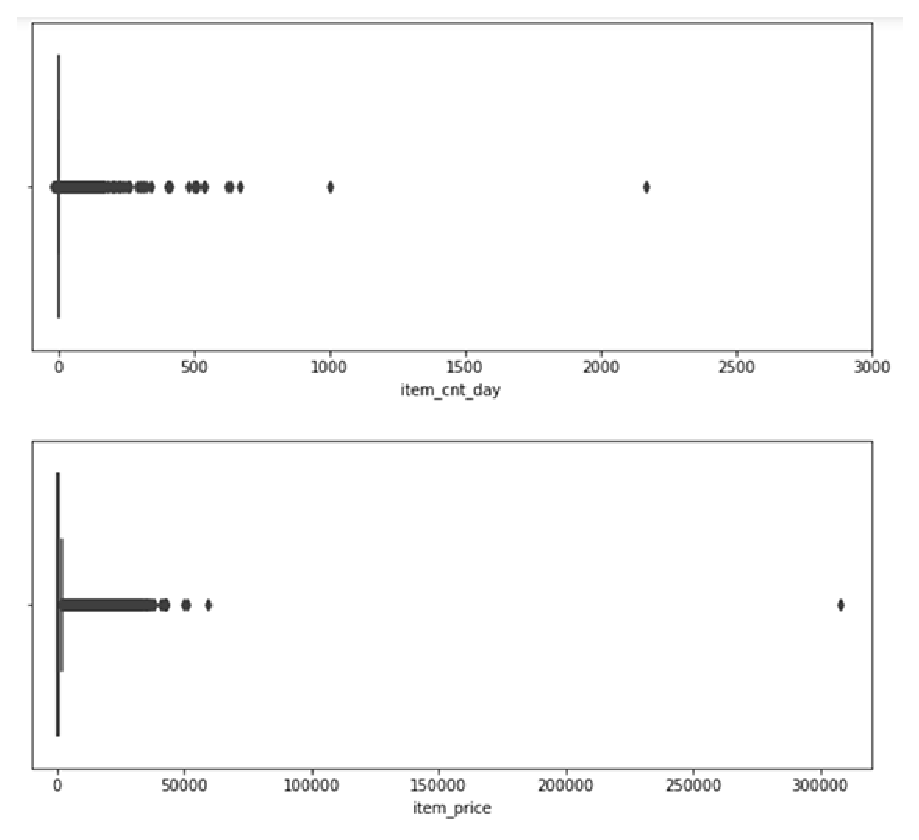
\includegraphics[width=10cm, height=8cm]{figures/outliers.eps}
			\caption{Outliers Data
			}\label{straddltimeScale}
		\end{figure}
		\begin{itemize}
			\item Filter duplicate data
			\smallskip
			\item Filter data with price less than zero
		\end{itemize}
	\end{slide}
	%%
	%%==========================================================================================
	%%==========================================================================================
	%%  
	\begin{slide}[toc=Process Shops Set]{Process Shops Set}
		\begin{itemize}
			\item Same shop name, different shop ID
			\begin{description}[type=0]
				\item 39 and 40,10 and 11,0 and 57, 58 and 1
			\end{description}
			\item Modify the ID based on the test
			\item Shop full name: shop's city-shop's type-shop's name
			\item Encode shops information
		\end{itemize}
		\begin{figure}[htb]
			\centering
			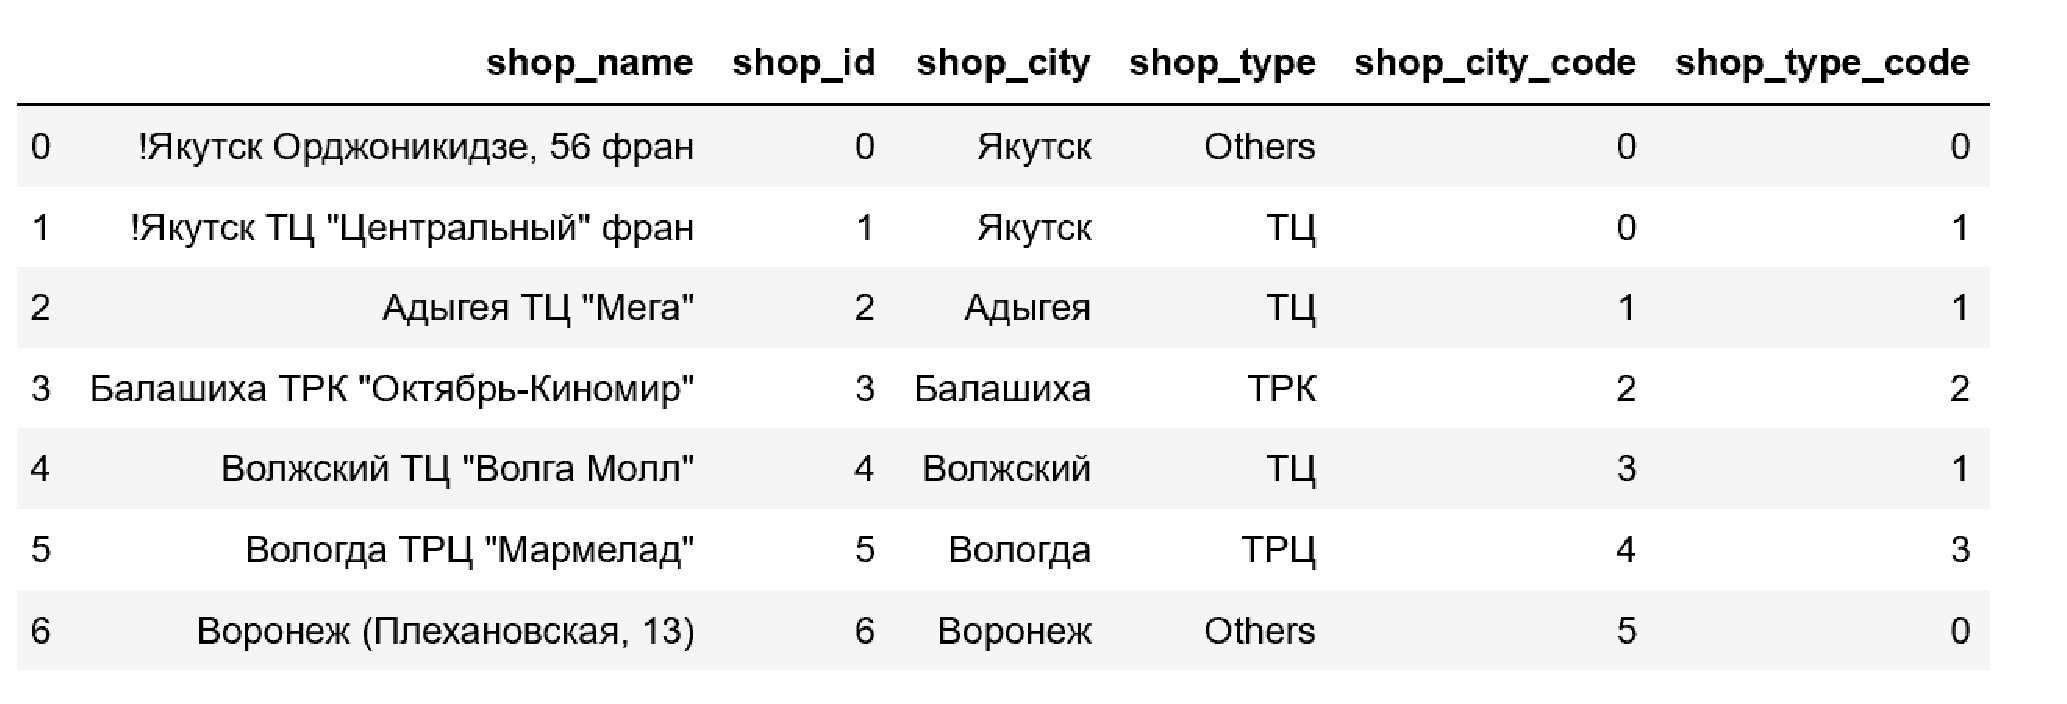
\includegraphics[width=17cm, height=6cm]{figures/shop encode.eps}
			\caption{Encode Shops Information
			}\label{straddltimeScale}
		\end{figure}
	\end{slide}
	%%
	%%==========================================================================================
	==================================
	%%  
	\begin{slide}[toc=Process Items Set]{Process Items Set}
		\begin{itemize}
			\item Same item name, different item ID
			\begin{description}[type=0]
				\item 2514 and 2558,2968 and 2970,5061 and 5063, 14537 and 14539,19465 and 19475,19579 and 19581
			\end{description}
			\item Modify the ID based on the test
		\end{itemize}
	\end{slide}
	%%
	%%==========================================================================================
	\begin{slide}[toc=Process Categories Set]{Process Categories Set}
		\begin{itemize}
			\item Shop full name: category's type-category's subtype
			\item Encode categories information
		\end{itemize}
		\begin{figure}[htb]
			\centering
			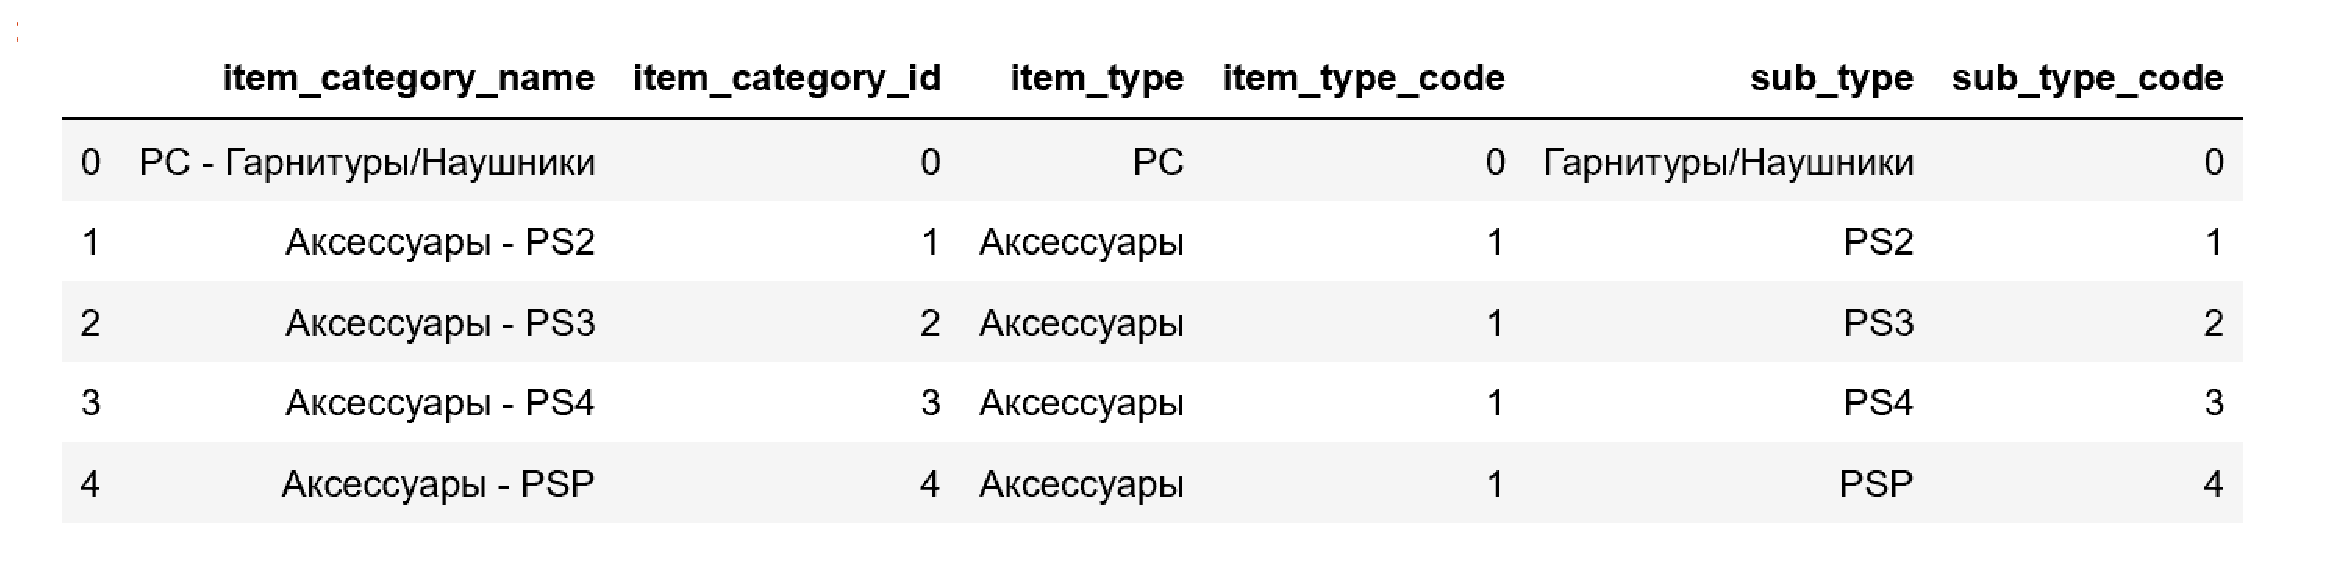
\includegraphics[width=19cm, height=5cm]{figures/category code.eps}
			\caption{Encode Categories Information
			}\label{straddltimeScale}
		\end{figure}
	\end{slide}
	%%
	%%==========================================================================================
	%%  
	\begin{slide}[toc=Sales Analysis]{Sales Analysis}
		\begin{figure}[htb]
			\centering
			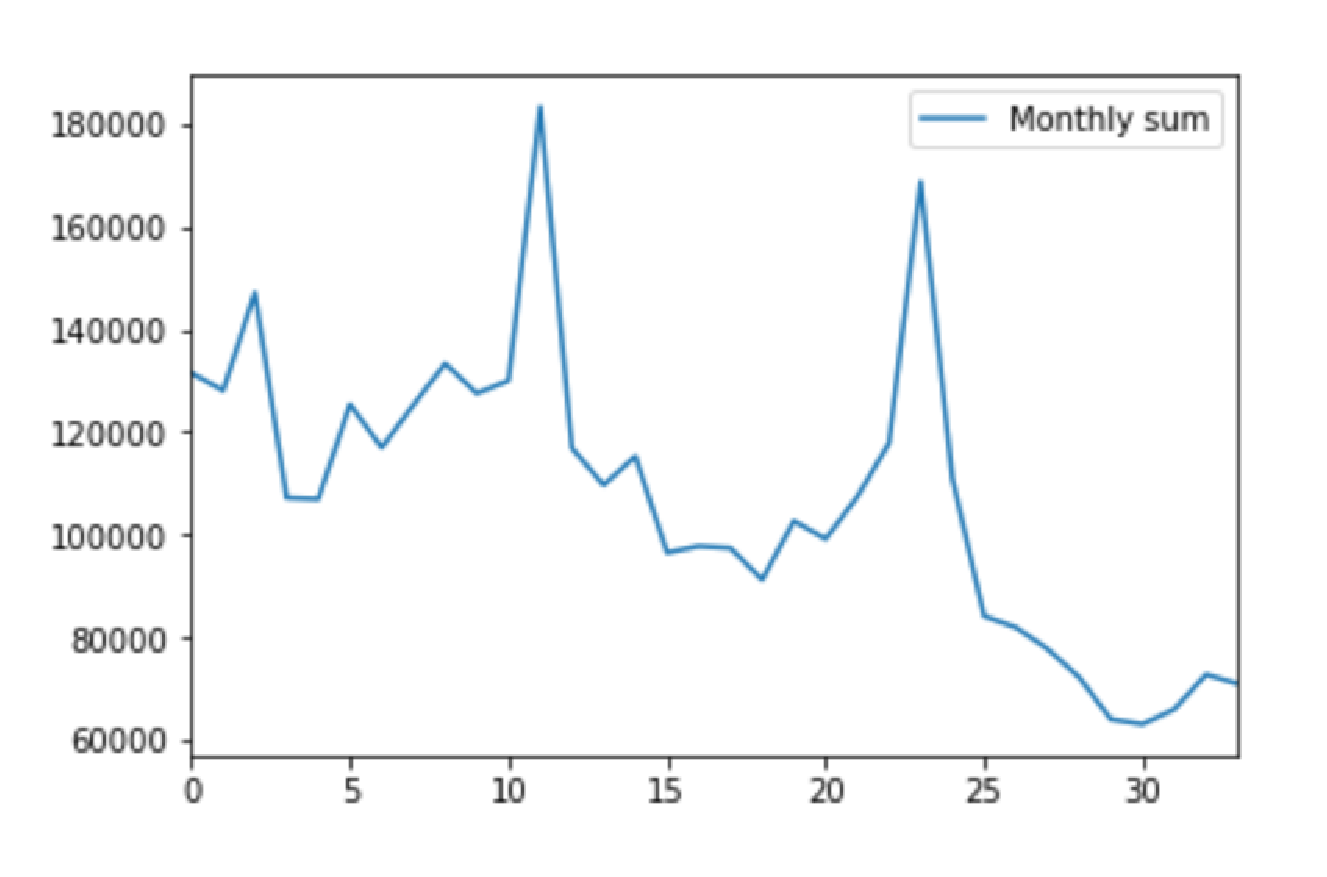
\includegraphics[width=15cm, height=10cm]{figures/sum.eps}
			\caption{Total Sales Over Time
			}\label{straddltimeScale}
		\end{figure}
	\end{slide}
	%%
	%%==========================================================================================
	%%==========================================================================================
	%%  
	\begin{slide}[toc=Closed Shops and Discontinued Products]{Closed Shops and Discontinued Products}
		
		\begin{itemize}
			\item new shops:9,20,36
			\item closed shops:0,1,8,11,13,17,23,27,29,30,32,33,40,43,51,54
		\end{itemize}
		\begin{figure}[htb]
			\centering
			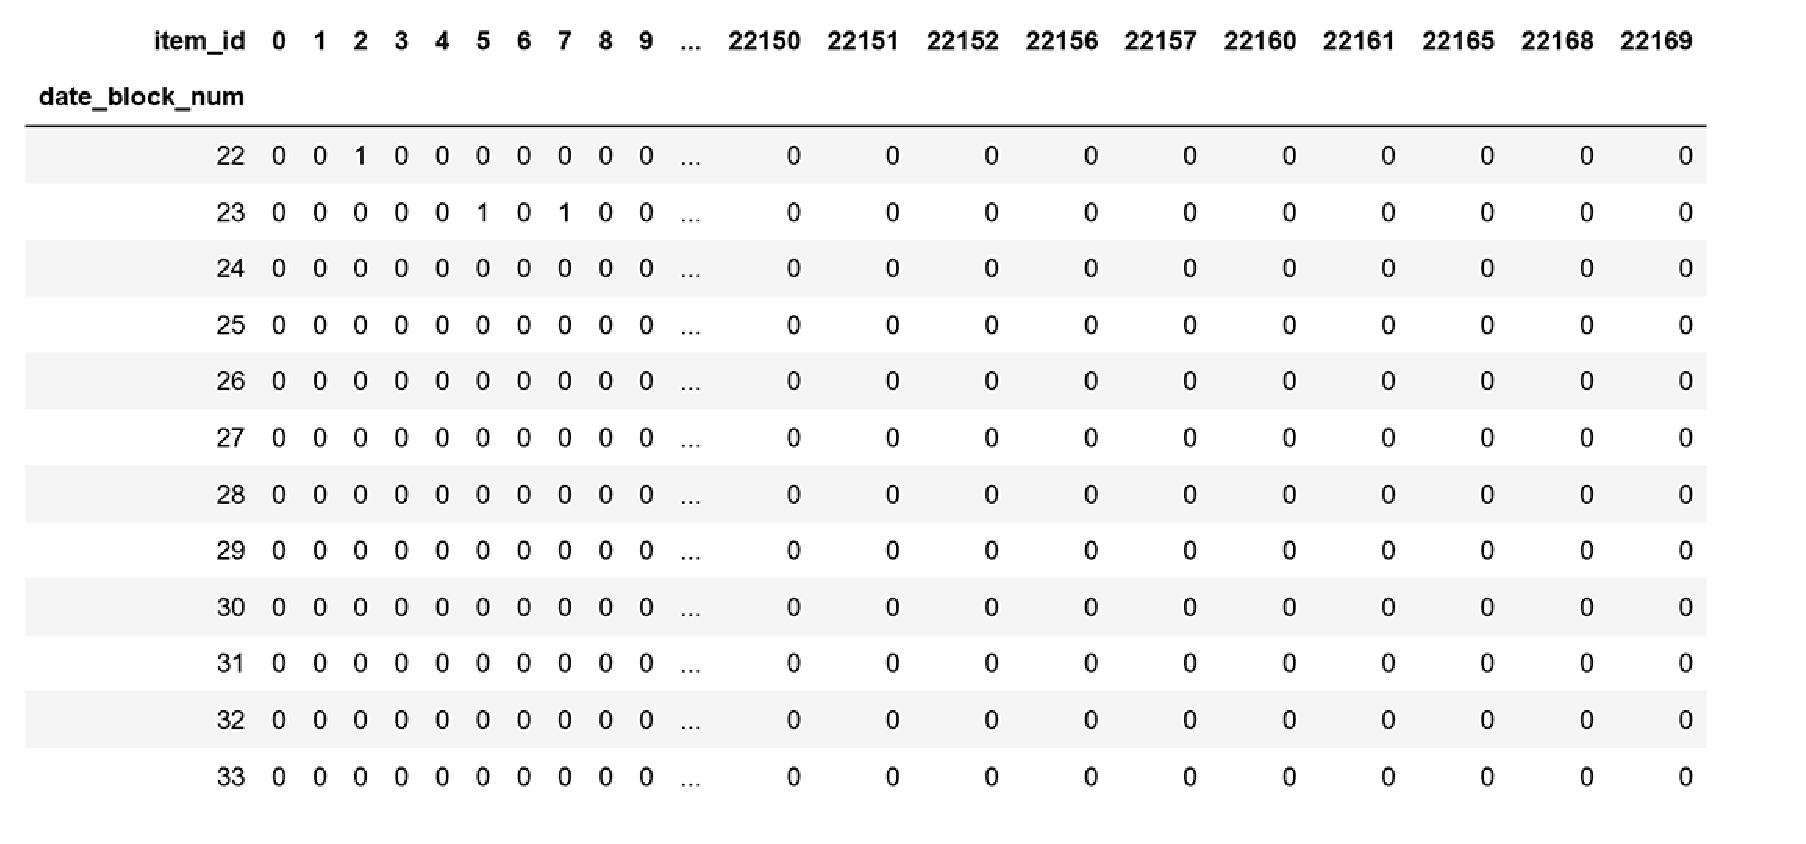
\includegraphics[width=18cm, height=8cm]{figures/stopitems.eps}
			\caption{Discontinued Products
			}\label{straddltimeScale}
		\end{figure}
	\end{slide}
	%%
	%%==========================================================================================
	===================================
	\section{Feature Selection}
	
	%%==========================================================================================
	%%  
	\begin{slide}[toc=Data Feature]{Data Feature}
		\begin{figure}[htb]
			\centering
			\includegraphics[width=20cm, height=8cm]{figures/feature.eps}
			\caption{Data Feature
			}\label{straddltimeScale}
		\end{figure}
		
	\end{slide}
	%%
	%%==========================================================================================
	%%  
	\begin{slide}[toc=Monthly Sales Feature]{Monthly Sales Feature}
		\begin{itemize}
			\item average monthly sales of items 
			\item average monthly sales of shops 
			\item average monthly sales of categories
			\item average monthly sales of types and subtypes
			\item average monthly sales of shop's city-item
			\item average monthly sales of shop's type-item
		\end{itemize}
	\end{slide}
	%%
	%%==========================================================================================
	%%  
	\begin{slide}[toc=Historical Feature]{Historical Feature}
		\begin{itemize}
			\item Historical delay:1,2,3,6,12
			\item Historical Feature: 
			\begin{description}[type=0]
				\item monthly sales of items 
				\item average monthly sales of shops 
				\item average monthly sales of items
				\item average monthly sales of categories
				\item average monthly sales of types and subtypes
				\item average monthly sales of shop's city-item
				\item average monthly sales of shop's type-item
			\end{description}
			\item Delete the records in first 12 months and NAN records
		\end{itemize}
	\end{slide}
	%%
	%%=======================================================
	
	\section{Modeling and Forecasting}
	\begin{slide}[toc=Feature Engineering,bm=]{Feature Engineering}
		\begin{figure}[htb]
			\centering
			\includegraphics[width=20cm, height=9cm]{figures/light.eps}
			\caption{Feature Importance
			}\label{straddltimeScale}
		\end{figure}
	\end{slide}
	%%==========================================================================================
	\begin{slide}[toc=Lightgbm,bm=]{Lightgbm}
		\begin{itemize}
			\item train set:date_block_num< 33\\   
			validation set:date_block_num == 33\\ 
			test set:date_block_num == 34
			\bigskip     
			\item score:0.93740
			\bigskip
			\item 3027/8738
		\end{itemize}
	\end{slide}
	%%============
	==============================================================================
	
	\begin{slide}[toc=Comparison,bm=]{Comparison}
		\begin{itemize}
			\item 1.0485→0.93740
			\bigskip    
			\item model and feature
			\begin{description}[type=0]
				\item LightGBM and XGBoost
				\smallskip    
				\item Add feature:historical feature
			\end{description}
		\end{itemize}
	\end{slide}
	%%===================================================================================================================================================
	
	%%==========================================================================================
	% TODO: Contact Page
	
\end{document}

\endinput
